\documentclass[11pt]{article}
\usepackage[left=2cm, right=2cm, top=2cm, bottom=2cm]{geometry} 
\usepackage{amsmath,amsthm,amssymb}
\usepackage{changepage}
\usepackage{dsfont}
\usepackage{graphicx}
\usepackage{titlesec}
\usepackage{array}
\usepackage{multirow}
\usepackage{booktabs}
\usepackage{listings}
\usepackage{fancyvrb}
\usepackage{hyperref}
 
\newcommand{\N}{\mathbb{N}}
\newcommand{\Z}{\mathbb{Z}}
\newcommand{\R}{\mathbb{R}}
\newcommand{\Q}{\mathbb{Q}}
\newcommand{\B}{\mathcal{R}}
\newcommand{\A}{\mathcal{A}}
\newcommand{\M}{\mathcal{M}}
\newcommand{\F}{\mathcal{F}}
\newcommand{\U}{\mathcal{U}}
\newcommand{\1}{\mathds{1}}

\def\code#1{\texttt{#1}}

\titleformat*{\section}{\large\bfseries}

% --------------------------------------------------------------
%                         Start here
% --------------------------------------------------------------	

\begin{document}

% --------------------------------------------------------------
%                            Title
% --------------------------------------------------------------	

\noindent
Blair Bilodeau 1001232230 \\
December 19, 2018 \\
STA2101 Final Project 

\begin{center}
	\textbf{An Analysis of Chicago Crime Data}
\end{center}


% --------------------------------------------------------------
%                         Introduction
% --------------------------------------------------------------	

\section{Introduction}

For this project I chose the option of analyzing some interesting data with Python. Using 3 datasets available from Kaggle, I investigated crime in Chicago from 2012 to 2016. The main goal of this is to explore data analysis in Python, specifically spatial plotting and multinomial logistic regression for determining relationships between crimes and the explanatory variables. Some questions I address are where crime occurs, what type of crime occurs, how crime in the area influences school quality, and how police station locations are related to crime hotspots.

The primary dataset used is \code{crimes}, which contains all reported incidents of crime in Chicago from 2012 to 2016. To supplement this, there is \code{schools}, which contains the progress report card of each public Chicago high school from the 2013-14 school year, and \code{police}, which contains location info for all Chicago police stations. These datasets have many fields, so I will only mention the critical ones that are used in a model. Appendix A contains a full list of fields for each one. All model output results are contained in Appendix C.

% --------------------------------------------------------------
%                         Crime Severity
% --------------------------------------------------------------

\section{Crime Severity}

The initial \code{crimes} file contains 1,456,714 rows, where each row corresponds to a crime being reported, but I removed 37,174 of these for missing location data. I also excluded crimes from 2017 since there were only 30, so it was logical to just consider years which were fully reported. The field \code{crimes[Primary Type]} details the main reason for a crime being reported, and I cleaned this up by removing some white space and grouping types such as ``NARCOTICS'' and ``OTHER NARCOTIC VIOLATION''. I split \code{crimes[Date]} into three fields for day, month, and year, and then dropped some redundant fields. A field that may have been useful is \code{crimes[Description]}, which contains a sentence describing the crime in more depth, but I decided there was too much variability in them to be practical for this analysis.

For this part of the analysis, I grouped the crime data by the field \code{crimes[Primary Type]} using my own subjective scale of severity, which can be found in Table~\ref{tab:severity}. Some of these were easy to rank (homicide most severe, non-criminal least severe), while others reveal my personal biases (some may rank prostitution offenses as more severe than I do). Nonetheless, I believe it worthwhile to determine how the covariates impact the severity of the crime committed.

\begin{table}[h]
	\small
	{\begin{tabular}{cl} \toprule
		\textbf{Severity} & \textbf{Primary Type} \\ \midrule
		1 & HOMICIDE, CRIMINAL SEXUAL ASSAULT, KIDNAPPING, HUMAN TRAFFICKING, \\
		  & OFFENSE INVOLVING CHILDREN \\ 
		2 & BURGLARY, THEFT, MOTOR VEHICLE THEFT, ROBBERY, ASSAULT, ARSON, \\
		  & SEX OFFENSE, BATTERY \\ 
		3 & NARCOTICS, STALKING, WEAPONS VIOLATION, CRIMINAL DAMAGE, \\
		  & CRIMINAL TRESPASS \\
		4 & GAMBLING, PROSTITUTION, OBSCENITY, LIQUOR LAW VIOLATION, \\
		  & PUBLIC PEACE VIOLATION, PUBLIC INDECENCY \\
		5 & INTIMIDATION, INTERFERENCE WITH PUBLIC OFFICER, DECEPTIVE PRACTICE \\
		6 & NON-CRIMINAL, OTHER OFFENSE \\ \bottomrule
	\end{tabular}} 
	\caption{Crime types categorized by severity level.}
	\label{tab:severity}
\end{table}

I then fit a multinomial logistic model to determine how severe a crime will be given covariates such as location, whether an arrest occurs, whether the crime is domestic related, where the crime occurred, and what time of year the crime occurred during. The results of this model are in Table 1-C, and reveal that with ``most severe'' as the reference category all of the covariates are significant for at least of one the possible outcomes.

Interestingly, we see evidence that an arrest will increase the probability of a lower severity, which I would guess is actually a reverse relationship and that low severity crimes are only reported when there is an easy arrest to be made. There is also a relationship to explore between crime location and severity, but the only location aspects I covered are in Section~\ref{sec:police}.

Most surprising is that there is an effect on severity by the date that the crime occurs. The sign of the coefficients suggests that a crime that is committed later in the year is more likely to be severe. Of course, one might expect this relationship to be non-linear, with a peak in severity occurring in the summer (see Toronto's ``Summer of Murder'' in 2018), and this cannot be captured by the current form of the model. 

% --------------------------------------------------------------
%                         Crime vs. School
% --------------------------------------------------------------

\section{School Safety}

Now, consider the \code{schools} dataset. Each row of this dataset corresponds to one of the 188 public high schools in Chicago. There are multiple fields that give a qualitative review of the school based on student and teacher surveys, as well as quantitative fields for test scores, attendance levels, and dropout rates. Most of the quantitative fields had very little data and so were not considered for this analysis. The fields \code{schools[Latitude]} and \code{schools[Longitude]} are labelled the other way around in the original file, so I swapped those back. 

The only survey question that got enough data from a significant proportion of schools is \code{schools[Safe]}, which rates how safe the school is on a scale of VERY WEAK, WEAK, NEUTRAL, STRONG, or VERY STRONG. After removing the schools with minimal data in the data cleaning process, I was left with 136. However, 18 of these still have NOT ENOUGH DATA in \code{schools[Safe]}. The question I am interested in is whether the number of crimes committed ``close'' to the school impacts how students and teachers rate the safety of the school. As I've already removed a significant number of schools for having many missing fields, I will use multiple imputation on these 18 schools. 

In order to determine the proximity of a crime to a school, I use an approximation of the Euclidean distance between two points determined by latitude and longitude as described by \\ \href{url}{https://andrew.hedges.name/experiments/haversine/}. Then, for each school I counted how many crimes were committed from 2012-2016 in a 0.5km and 1km radius around the school, and used this along with the other covariates to fit a multinomial logistic regression model with \code{schools[Safe]} as the response variable. The output of this model is in Table 2-C, where you can see that lots of the covariates are not significant, including the number of crimes committed in a certain radius. So, I fit a reduced model, which is displayed in Table 3-C and now has all coefficients significantly non-zero. 

I performed a likelihood ratio test on the reduced model and the full model, obtaining a test statistic of $G^2 = 40.21$ which on 28 degrees of freedom corresponds to a p value of 0.0633. Thus, I do not have evidence to conclude that the reduced model is different from the full model, so I will use the reduced model. With this, I impute the value of \code{schools[Safe]} for the 18 schools which didn't have enough data by simulating a multinomial random variable with the respective predicted probabilities. In order to account for the additional error in the imputation, I repeat this process 1000 times, each time recalculating the full model on all 136 datapoints. From each iteration, I obtain confidence intervals for each coefficient, and then I use the bootstrap average lower and upper bound to get my final confidence intervals for the coefficients. The results of this are in Table 4-C.

The main result from this process is that the bootstrapped confidence interval for number of crimes committed within 0.5km and 1km still contains zero after imputation. Thus, I do not have evidence to conclude that this is significant in the model, which suggests that it does not impact how students and teachers rate the safety of their school in a survey. Python's \code{statsmodels.MNLogit} function mysteriously did not like when I added in more columns at different radius sizes, but I ran it a few times swapping them out for each other and got the same results.

% --------------------------------------------------------------
%                         Crimes vs. Police
% --------------------------------------------------------------

\section{Police Stations} \label{sec:police}

\noindent
Finally, consider the \code{police} dataset. This is the smallest dataset, with only 23 rows -- one for each police station in Chicago. The only fields I care about from this dataset are \code{police[Latitude]} and \code{police[Longitude]}.  The null hypothesis I wish to test here is that crime location is not influenced by where police stations are. This is a little nebulous, so first I compare these visually. In Figure~\ref{fig:location1}, it's clear that more crimes are committed in the very center of the city as well as to the West. The police stations (blue dots) also seem to be slightly more concentrated in the center of the city than at the edges. 

\begin{figure}[h]
	\centering
	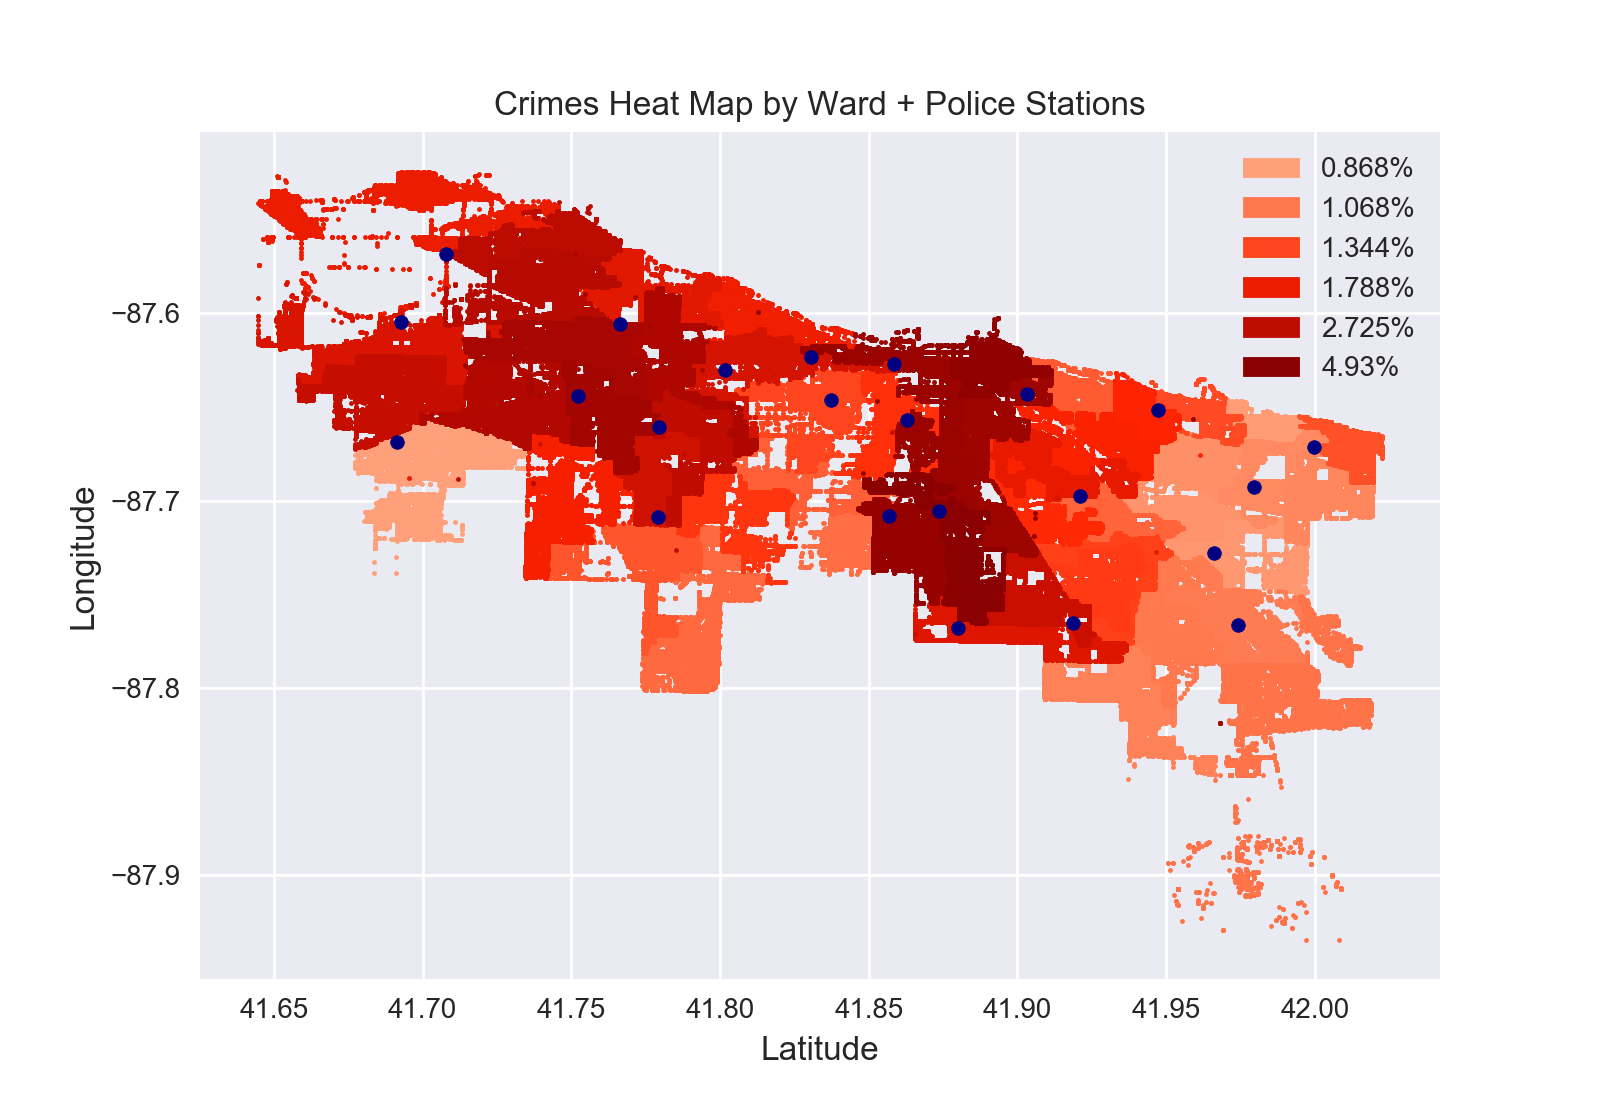
\includegraphics[width=140mm, height=100mm]{crime_locations.png}
	\caption{Location of all crimes reported along with the police stations in Chicago, colour coded by the percentage of crimes from the ward where the crime was reported. Legend is just a sample of colours to give an idea of scale.}
	\label{fig:location1}
\end{figure}

Explicitly, I calculate the number of crimes committed within 1km (inner radius) of each police station and the number of crimes committed between 1km and $\sqrt{2}$km (outer radius) from each police station. The $\sqrt{2}$ is so that this strip has the same area as a 1km circle, that is $\pi\text{km}^2$. I repeat this for 100 iterations of bootstrapping the crime location data, each time computing the mean paired difference of counts.

The value computed is \code{inner radius} $-$ \code{outer radius}, which gives a bootstrap 95\% confidence interval of (1586, 1631). Thus, I reject the null hypothesis and conclude that more crimes are reported close to a police station than farther away. This is not unreasonable, since presumably there are more police present in the inner radius to bear witness to a crime than the outer radius .

% --------------------------------------------------------------
%                         Conclusions
% --------------------------------------------------------------

\section{Conclusions}

Ultimately, I answered three questions from the data available, all at a 95\% significance level. The first of these is which covariates influence the severity of crimes committed, which I determined to be whether the crime led to an arrest, where the crime occurred, and the time of year when the crime occurred. Next, I found the number of crimes committed in different radii around each public high school. For the schools with missing data, I used multiple imputation to fill in the survey ranking of school safety. The imputed data led me to conclude that there is no evidence that the number of crimes committed near a school impacts how students and teachers rate the school's safety. I also computed how many crimes were committed in a radius directly around each police station and a doughnut shape for the strip just outside this inner radius. I concluded that there are significantly more crimes committed close to the police station than just outside the inner radius.

To me, the most interesting results of this analysis involved the location data. Future analysis might involve more visualizations, and perhaps fitting something like a poisson point process to measure the dispersion of crimes. In addition to the statistical analysis, I learned how to compute these models using Python, which provided just as much versatility as R with enough experimentation.

% --------------------------------------------------------------
%                         Appendices
% --------------------------------------------------------------

\section*{Appendix A - Datasets}

The \code{crimes} dataset can be accessed from: \\
\href{https://www.kaggle.com/currie32/crimes-in-chicago#Chicago_Crimes_2012_to_2017.csv}{https://www.kaggle.com/currie32/crimes-in-chicago\#Chicago\_Crimes\_2012\_to\_2017.csv}. \\
The following field descriptions are from: \\
\href{url}{https://www.kaggle.com/currie32/crimes-in-chicago/home}. 

\begin{Verbatim}[fontsize=\small]
Case Number - The Chicago Police Department RD Number (Records Division Number), which is unique 
to the incident.

Date - Date when the incident occurred. this is sometimes a best estimate.

Block - The partially redacted address where the incident occurred, placing it on the same block 
as the actual address.

IUCR - The Illinois Unifrom Crime Reporting code. This is directly linked to the Primary Type 
and Description. See the list of IUCR codes at https://data.cityofchicago.org/d/c7ck-438e.

Primary Type - The primary description of the IUCR code.

Description - The secondary description of the IUCR code, a subcategory of the primary description.

Location Description - Description of the location where the incident occurred.

Arrest - Indicates whether an arrest was made.

Domestic - Indicates whether the incident was domestic-related as defined by the Illinois Domestic 
Violence Act.

Beat - Indicates the beat where the incident occurred. A beat is the smallest police geographic 
area -– each beat has a dedicated police beat car. Three to five beats make up a police sector, 
and three sectors make up a police district. The Chicago Police Department has 22 police districts. 
See the beats at https://data.cityofchicago.org/d/aerh-rz74.

District - Indicates the police district where the incident occurred. 
See the districts at https://data.cityofchicago.org/d/fthy-xz3r.

Ward - The ward (City Council district) where the incident occurred. 
See the wards at https://data.cityofchicago.org/d/sp34-6z76.

Community Area - Indicates the community area where the incident occurred. Chicago has 77 community 
areas. See the community areas at https://data.cityofchicago.org/d/cauq-8yn6.

FBI Code - Indicates the crime classification as outlined in the FBI's National Incident-Based 
Reporting System (NIBRS). See the Chicago Police Department listing of these classifications 
at http://gis.chicagopolice.org/clearmap_crime_sums/crime_types.html.

X Coordinate - The x coordinate of the location where the incident occurred in State Plane Illinois 
East NAD 1983 projection. This location is shifted from the actual location for partial redaction but 
falls on the same block.

Y Coordinate - The y coordinate of the location where the incident occurred in State Plane Illinois 
East NAD 1983 projection. This location is shifted from the actual location for partial redaction but 
falls on the same block.

Year - Year the incident occurred.

Updated On - Date and time the record was last updated.

Latitude - The latitude of the location where the incident occurred. This location is shifted 
from the actual location for partial redaction but falls on the same block.

Longitude - The longitude of the location where the incident occurred. This location is shifted 
from the actual location for partial redaction but falls on the same block.

Location - The location where the incident occurred in a format that allows for creation of maps and 
other geographic operations on this data portal. This location is shifted from the actual location 
for partial redaction but falls on the same block.
\end{Verbatim}

\noindent
The \code{schools} dataset can be accessed from: \\
\href{https://www.kaggle.com/chicago/chicago-public-schools-data#chicago-public-schools-high-school-progress-report-2013-2014.csv}{https://www.kaggle.com/chicago/chicago-public-schools-data\#chicago-public-schools-high-school-progress-report-2013-2014.csv}. There are alot of column names, and most are pretty self-explanatory, so I will just list them.

\begin{Verbatim}[fontsize=\small]
School ID 
Name of School
Street Address
City
State
ZIP Code
Phone Number
Website
Blue Ribbon Award
CPS Performance Policy Level
CPS Performance Policy Status
Probation Length
My Voice, My School Overall Rating
Student Response Rate
Teacher Response Rate
Involved Family
Supportive Environment
Ambitious Instruction
Effective Leaders
Collaborative Teachers
Safe
School Community
Parent-Teacher Partnership
Quality of Facilities
Healthy Schools Certification
Creative Schools Certification
NWEA Reading Growth Percentile All Grades
NWEA Reading Growth Percentile Grade 3
NWEA Reading Growth Percentile Grade 4
NWEA Reading Growth Percentile Grade 5
NWEA Reading Growth Percentile Grade 6
NWEA Reading Growth Percentile Grade 7
NWEA Reading Growth Percentile Grade 8
NWEA Math Growth All Grades
NWEA Math Growth Grade 3
NWEA Math Growth Grade 4
NWEA Math Growth Grade 5
NWEA Math Growth Grade 6
NWEA Math Growth Grade 7
NWEA Math Growth Grade 8
NWEA Reading Attainment Percentile All Grades
NWEA Reading Attainment Percentile Grade 2
NWEA Reading Attainment Percentile Grade 3
NWEA Reading Attainment Percentile Grade 4
NWEA Reading Attainment Percentile Grade 5
NWEA Reading Attainment Percentile Grade 6
NWEA Reading Attainment Percentile Grade 7
NWEA Reading Attainment Percentile Grade 8
NWEA Math Attainment Percentile All Grades
NWEA Math Attainment Percentile Grade 2
NWEA Math Attainment Percentile Grade 3
NWEA Math Attainment Percentile Grade 4
NWEA Math Attainment Percentile Grade 5
NWEA Math Attainment Percentile Grade 6
NWEA Math Attainment Percentile Grade 7
NWEA Math Attainment Percentile Grade 8
EPAS Growth Percentile
EXPLORE Growth Percentile Grade 9
Plan Growth Percentile Grade 10
ACT Growth Percentile Grade 11
EPAS Attainment Percentile
EXPLORE Attainment Percentile Grade 9
PLAN Attainment Percentile Grade 10
Grade ACT Attainment Percentile Grade 11
EXPLORE Spring 2013 Average Grade 9
EXPLORE Spring 2013 Average Grade 10
EXPLORE Fall 2011 Average Grade 9
PLAN Fall 2012 Average Grade 10
ACT Spring 2013 Average Grade 11',
Freshmen-on-Track Rate Percentage 2013
Freshmen-on-Track Rate Percentage 2012
4-Year Graduation Rate Percentage 2013
4-Year Graduation Rate Percentage 2012
5-Year Graduation Rate Percentage 2013
5-Year Graduation Rate Percentage 2012
College Enrollment Rate Percentage 2013
College Enrollment Rate Percentage 2012
College Persistence Rate Percentage 2013
College Persistence Rate Percentage 2012
Suspensions Per 100 2013
Suspensions Per 100 2012
Percentage of Misconducts Resulting in Suspension 2013
Percentage of Misconducts Resulting in Suspension 2012
Average Length of Suspensions 2013
Average Length of Suspensions 2012
Student Attendance Percentage 2013
Student Attendance Percentage 2012
Teacher Attendance Percentage 2013
Teacher Attendance Percentage 2012
Gr3-8 On-Track Percentage 2013
One-Year DropOut Rate Percentage 2013
One-Year DropOut Rate Percentage 2012
X Coordinate
Y Coordinate
Longitude
Latitude
Location
\end{Verbatim}

\noindent
The \code{police} dataset can be accessed from:
\href{https://www.kaggle.com/chicago/chicago-police-stations}{https://www.kaggle.com/chicago/chicago-police-stations}. Again, I'm not so interested in most of these columns, so I will just list them.

\begin{Verbatim}[fontsize=\small]
DISTRICT
DISTRICT NAME
ADDRESS
CITY
STATE
ZIP
WEBSITE
PHONE
FAX
TTY
X COORDINATE
Y COORDINATE
LATITUDE
LONGITUDE
LOCATION
\end{Verbatim}

\section*{Appendix B - Code}
The Python file is quite long and wouldn't format nicely in this PDF file, so please see the attached BlairBilodeauSTA2101FinalProject.py file in the email.

\newpage
\section*{Appendix C - Results}

Table 1-C: Crime Severity Multinomial Logistic Model
\begin{Verbatim}[fontsize=\tiny]
MNLogit Regression Results                          
==============================================================================
Dep. Variable:         Crime Severity   No. Observations:              1419517
Model:                        MNLogit   Df Residuals:                  1419482
Method:                           MLE   Df Model:                           30
Date:                Sat, 24 Nov 2018   Pseudo R-squ.:                 0.09873
Time:                        12:08:38   Log-Likelihood:            -1.4036e+06
converged:                       True   LL-Null:                   -1.5574e+06
                                        LLR p-value:                     0.000
====================================================================================
Crime Severity=2       coef    std err          z      P>|z|      [0.025      0.975]
------------------------------------------------------------------------------------
Arrest              -0.1151      0.019     -6.093      0.000      -0.152      -0.078
Domestic            -0.8151      0.015    -54.260      0.000      -0.845      -0.786
Year                -0.0070      0.004     -1.929      0.054      -0.014       0.000
Latitude             1.6651      0.099     16.817      0.000       1.471       1.859
Longitude            0.5903      0.104      5.683      0.000       0.387       0.794
Month                0.0131      0.002      6.180      0.000       0.009       0.017
Day                  0.0064      0.001      7.977      0.000       0.005       0.008
------------------------------------------------------------------------------------
Crime Severity=3       coef    std err          z      P>|z|      [0.025      0.975]
------------------------------------------------------------------------------------
Arrest               1.7122      0.019     89.942      0.000       1.675       1.749
Domestic            -2.2771      0.017   -135.238      0.000      -2.310      -2.244
Year                -0.0682      0.004    -18.253      0.000      -0.076      -0.061
Latitude            -0.3517      0.102     -3.460      0.001      -0.551      -0.152
Longitude           -1.7625      0.107    -16.519      0.000      -1.972      -1.553
Month                0.0013      0.002      0.579      0.562      -0.003       0.006
Day                  0.0058      0.001      7.094      0.000       0.004       0.007
------------------------------------------------------------------------------------
Crime Severity=4       coef    std err          z      P>|z|      [0.025      0.975]
------------------------------------------------------------------------------------
Arrest               3.4872      0.027    131.002      0.000       3.435       3.539
Domestic            -3.3843      0.050    -67.178      0.000      -3.483      -3.286
Year                -0.1063      0.005    -21.222      0.000      -0.116      -0.097
Latitude            -0.6723      0.137     -4.900      0.000      -0.941      -0.403
Longitude           -2.7475      0.143    -19.169      0.000      -3.028      -2.467
Month                0.0078      0.003      2.698      0.007       0.002       0.013
Day                  0.0063      0.001      5.812      0.000       0.004       0.008
------------------------------------------------------------------------------------
Crime Severity=5       coef    std err          z      P>|z|      [0.025      0.975]
------------------------------------------------------------------------------------
Arrest               0.2259      0.021     10.807      0.000       0.185       0.267
Domestic            -3.9168      0.040    -98.234      0.000      -3.995      -3.839
Year                 0.0702      0.004     17.190      0.000       0.062       0.078
Latitude             3.5473      0.110     32.253      0.000       3.332       3.763
Longitude            3.2869      0.116     28.340      0.000       3.060       3.514
Month                0.0003      0.002      0.122      0.903      -0.004       0.005
Day                  0.0009      0.001      0.964      0.335      -0.001       0.003
------------------------------------------------------------------------------------
Crime Severity=6       coef    std err          z      P>|z|      [0.025      0.975]
------------------------------------------------------------------------------------
Arrest               0.2904      0.020     14.228      0.000       0.250       0.330
Domestic            -0.1294      0.017     -7.831      0.000      -0.162      -0.097
Year                -0.0338      0.004     -8.467      0.000      -0.042      -0.026
Latitude             0.5739      0.109      5.272      0.000       0.361       0.787
Longitude           -0.5190      0.114     -4.546      0.000      -0.743      -0.295
Month               -0.0056      0.002     -2.382      0.017      -0.010      -0.001
Day                  0.0023      0.001      2.574      0.010       0.001       0.004
====================================================================================  
\end{Verbatim}

\newpage
\noindent 
Table 2-C: School Safety Multinomial Logistic Model
\begin{Verbatim}[fontsize=\tiny]
MNLogit Regression Results                          
==============================================================================
Dep. Variable:                   Safe   No. Observations:                  118
Model:                        MNLogit   Df Residuals:                       70
Method:                           MLE   Df Model:                           44
Date:                Sat, 24 Nov 2018   Pseudo R-squ.:                  0.4531
Time:                        21:26:23   Log-Likelihood:                -84.131
converged:                       True   LL-Null:                       -153.83
                                        LLR p-value:                 7.608e-12
============================================================================================================
                             Safe=STRONG       coef    std err          z      P>|z|      [0.025      0.975]
------------------------------------------------------------------------------------------------------------
Student Response Rate                       -0.0038      0.027     -0.142      0.887      -0.056       0.048
Teacher Response Rate                       -0.0130      0.022     -0.604      0.546      -0.055       0.029
EPAS Growth Percentile                      -0.0061      0.013     -0.466      0.642      -0.032       0.020
EPAS Attainment Percentile                   0.2829      0.110      2.571      0.010       0.067       0.499
Grade ACT Attainment Percentile Grade 11    -0.1077      0.145     -0.743      0.458      -0.392       0.176
ACT Spring 2013 Average Grade 11            -1.1330      1.057     -1.072      0.284      -3.204       0.938
Student Attendance Percentage 2013           0.0440      0.071      0.623      0.534      -0.094       0.182
One-Year DropOut Rate Percentage 2013        0.0667      0.038      1.755      0.079      -0.008       0.141
Latitude                                    12.5131      4.802      2.606      0.009       3.101      21.925
Longitude                                    5.8556      2.299      2.547      0.011       1.350      10.361
Crimes Committed 0.5km                    -3.49e-05      0.000     -0.128      0.898      -0.001       0.000
Crimes Committed 1km                     -2.876e-05      0.000     -0.221      0.825      -0.000       0.000
------------------------------------------------------------------------------------------------------------
                        Safe=VERY STRONG       coef    std err          z      P>|z|      [0.025      0.975]
------------------------------------------------------------------------------------------------------------
Student Response Rate                       -0.0117      0.086     -0.136      0.892      -0.181       0.157
Teacher Response Rate                        0.0591      0.108      0.547      0.584      -0.153       0.271
EPAS Growth Percentile                      -0.0287      0.033     -0.870      0.384      -0.093       0.036
EPAS Attainment Percentile                  -0.0470      0.331     -0.142      0.887      -0.696       0.602
Grade ACT Attainment Percentile Grade 11    -0.2014      0.353     -0.570      0.569      -0.894       0.491
ACT Spring 2013 Average Grade 11             3.3370      2.203      1.515      0.130      -0.981       7.655
Student Attendance Percentage 2013           0.1301      0.260      0.499      0.618      -0.381       0.641
One-Year DropOut Rate Percentage 2013        0.2328      0.132      1.757      0.079      -0.027       0.492
Latitude                                    -1.3604     10.328     -0.132      0.895     -21.603      18.882
Longitude                                    0.1280      4.949      0.026      0.979      -9.572       9.828
Crimes Committed 0.5km                      -0.0008      0.001     -0.618      0.537      -0.003       0.002
Crimes Committed 1km                        -0.0001      0.000     -0.297      0.766      -0.001       0.001
------------------------------------------------------------------------------------------------------------
                    	Safe=VERY WEAK       coef    std err          z      P>|z|      [0.025      0.975]
------------------------------------------------------------------------------------------------------------
Student Response Rate                       -0.1712      0.148     -1.158      0.247      -0.461       0.119
Teacher Response Rate                       -0.0121      0.199     -0.061      0.951      -0.402       0.378
EPAS Growth Percentile                       0.0730      0.071      1.022      0.307      -0.067       0.213
EPAS Attainment Percentile                  -2.8732      2.257     -1.273      0.203      -7.297       1.551
Grade ACT Attainment Percentile Grade 11     2.7547      2.388      1.153      0.249      -1.926       7.436
ACT Spring 2013 Average Grade 11             0.0001      4.945      3e-05      1.000      -9.692       9.692
Student Attendance Percentage 2013          -0.3628      0.450     -0.806      0.420      -1.245       0.519
One-Year DropOut Rate Percentage 2013       -0.1222      0.279     -0.439      0.661      -0.669       0.424
Latitude                                   -58.9888     39.143     -1.507      0.132    -135.707      17.729
Longitude                                  -28.5170     18.862     -1.512      0.131     -65.485       8.451
Crimes Committed 0.5km                       0.0018      0.002      1.079      0.281      -0.002       0.005
Crimes Committed 1km                        -0.0004      0.001     -0.749      0.454      -0.001       0.001
------------------------------------------------------------------------------------------------------------
                               Safe=WEAK       coef    std err          z      P>|z|      [0.025      0.975]
------------------------------------------------------------------------------------------------------------
Student Response Rate                       -0.0385      0.026     -1.469      0.142      -0.090       0.013
Teacher Response Rate                       -0.0082      0.025     -0.323      0.746      -0.058       0.042
EPAS Growth Percentile                       0.0102      0.015      0.695      0.487      -0.019       0.039
EPAS Attainment Percentile                  -0.1710      0.137     -1.244      0.214      -0.440       0.099
Grade ACT Attainment Percentile Grade 11     0.0803      0.221      0.363      0.716      -0.353       0.513
ACT Spring 2013 Average Grade 11            -0.2075      1.239     -0.167      0.867      -2.636       2.221
Student Attendance Percentage 2013          -0.0524      0.052     -1.002      0.316      -0.155       0.050
One-Year DropOut Rate Percentage 2013       -0.0986      0.040     -2.443      0.015      -0.178      -0.019
Latitude                                   -11.3823      5.074     -2.243      0.025     -21.327      -1.438
Longitude                                   -5.5696      2.442     -2.280      0.023     -10.356      -0.783
Crimes Committed 0.5km                    5.189e-05      0.000      0.121      0.903      -0.001       0.001
Crimes Committed 1km                     -3.292e-06      0.000     -0.028      0.977      -0.000       0.000
============================================================================================================   
\end{Verbatim}

\newpage
\noindent
Table 3-C: School Safety Multinomial Logistic Reduced Model
\begin{Verbatim}[fontsize=\tiny]
MNLogit Regression Results                          
==============================================================================
Dep. Variable:                   Safe   No. Observations:                  118
Model:                        MNLogit   Df Residuals:                       98
Method:                           MLE   Df Model:                           16
Date:                Sat, 24 Nov 2018   Pseudo R-squ.:                  0.3224
Time:                        21:43:25   Log-Likelihood:                -104.24
converged:                       True   LL-Null:                       -153.83
                                        LLR p-value:                 4.914e-14
=========================================================================================================
                          Safe=STRONG       coef    std err          z      P>|z|      [0.025      0.975]
---------------------------------------------------------------------------------------------------------
Student Response Rate                    -0.0092      0.022     -0.415      0.678      -0.053       0.034
EPAS Attainment Percentile                0.0467      0.015      3.116      0.002       0.017       0.076
One-Year DropOut Rate Percentage 2013     0.0551      0.029      1.919      0.055      -0.001       0.111
Latitude                                  7.6611      3.974      1.928      0.054      -0.128      15.450
Longitude                                 3.6813      1.901      1.937      0.053      -0.044       7.407
---------------------------------------------------------------------------------------------------------
                     Safe=VERY STRONG       coef    std err          z      P>|z|      [0.025      0.975]
---------------------------------------------------------------------------------------------------------
Student Response Rate                     0.0268      0.048      0.561      0.575      -0.067       0.120
EPAS Attainment Percentile                0.1235      0.032      3.881      0.000       0.061       0.186
One-Year DropOut Rate Percentage 2013     0.1854      0.066      2.810      0.005       0.056       0.315
Latitude                                 -3.0168      6.593     -0.458      0.647     -15.939       9.906
Longitude                                -1.3134      3.140     -0.418      0.676      -7.469       4.842
---------------------------------------------------------------------------------------------------------
                       Safe=VERY WEAK       coef    std err          z      P>|z|      [0.025      0.975]
---------------------------------------------------------------------------------------------------------
Student Response Rate                    -0.0025      0.056     -0.045      0.964      -0.112       0.107
EPAS Attainment Percentile               -0.2092      0.136     -1.534      0.125      -0.476       0.058
One-Year DropOut Rate Percentage 2013    -0.0458      0.073     -0.625      0.532      -0.189       0.098
Latitude                                -22.0762     11.050     -1.998      0.046     -43.734      -0.419
Longitude                               -10.5304      5.270     -1.998      0.046     -20.860      -0.201
---------------------------------------------------------------------------------------------------------
                            Safe=WEAK       coef    std err          z      P>|z|      [0.025      0.975]
---------------------------------------------------------------------------------------------------------
Student Response Rate                    -0.0412      0.021     -1.994      0.046      -0.082      -0.001
EPAS Attainment Percentile               -0.1356      0.039     -3.509      0.000      -0.211      -0.060
One-Year DropOut Rate Percentage 2013    -0.0828      0.035     -2.341      0.019      -0.152      -0.013
Latitude                                -10.6719      4.637     -2.301      0.021     -19.761      -1.583
Longitude                                -5.1489      2.217     -2.322      0.020      -9.494      -0.804
=========================================================================================================
\end{Verbatim}

\newpage
\noindent
Table 4-C: School Safety Multinomial Logistic Imputed Bootstrap Confidence Intervals
\begin{Verbatim}[fontsize=\tiny]
==================================================================
                             Safe=STRONG     [0.025      0.975]         
------------------------------------------------------------------
Student Response Rate                       -0.0553      0.0361     
Teacher Response Rate                       -0.0505      0.0303     
EPAS Growth Percentile                      -0.0306      0.0182
EPAS Attainment Percentile                   0.0536      0.4682
Grade ACT Attainment Percentile Grade 11    -0.3319      0.1973
ACT Spring 2013 Average Grade 11            -3.2238      0.5732
Student Attendance Percentage 2013          -0.0928      0.1792
One-Year DropOut Rate Percentage 2013       -0.0127      0.1295 
Latitude                                     2.2649     20.2106
Longitude                                    0.928       9.4907
Crimes Committed 0.5km                      -0.0005      0.0005
Crimes Committed 1km                        -0.0003      0.0002
------------------------------------------------------------------
                        Safe=VERY STRONG     [0.025      0.975]         
------------------------------------------------------------------
Student Response Rate                       -0.1785      0.0885
Teacher Response Rate                       -0.1156      0.2305
EPAS Growth Percentile                      -0.0738      0.0334
EPAS Attainment Percentile                  -0.688       0.4663
Grade ACT Attainment Percentile Grade 11    -0.6902      0.5267
ACT Spring 2013 Average Grade 11            -0.8881      6.2761 
Student Attendance Percentage 2013          -0.3395      0.5248 
One-Year DropOut Rate Percentage 2013       -0.0371      0.403  
Latitude                                   -22.5398     14.6637
Longitude                                  -10.1751      7.6211
Crimes Committed 0.5km                      -0.0029      0.0015
Crimes Committed 1km                        -0.0007      0.0006
------------------------------------------------------------------
                         Safe=VERY WEAK      [0.025      0.975]         
------------------------------------------------------------------
Student Response Rate                       -0.182       0.0589
Teacher Response Rate                       -0.1802      0.1666
EPAS Growth Percentile                      -0.031       0.0819
EPAS Attainment Percentile                  -1.8504      0.0805
Grade ACT Attainment Percentile Grade 11    -0.7686      2.0723
ACT Spring 2013 Average Grade 11            -5.7878      8.1617
Student Attendance Percentage 2013          -0.573       0.1335
One-Year DropOut Rate Percentage 2013       -0.393       0.1686
Latitude                                   -71.4799      5.0597
Longitude                                  -34.1409      2.3914
Crimes Committed 0.5km                      -0.0015      0.0037
Crimes Committed 1km                        -0.001       0.0005
------------------------------------------------------------------
                           Safe=WEAK         [0.025      0.975]         
------------------------------------------------------------------
Student Response Rate                       -0.0817      0.0081
Teacher Response Rate                       -0.0553      0.0368
EPAS Growth Percentile                      -0.0175      0.0352
EPAS Attainment Percentile                  -0.3826      0.1029
Grade ACT Attainment Percentile Grade 11    -0.3588      0.4125
ACT Spring 2013 Average Grade 11            -2.1312      2.2394
Student Attendance Percentage 2013          -0.1619      0.0387
One-Year DropOut Rate Percentage 2013       -0.179      -0.0231
Latitude                                   -20.1468     -0.9197
Longitude                                   -9.7418     -0.5183
Crimes Committed 0.5km                      -0.0007      0.0008
Crimes Committed 1km                        -0.0002      0.0002
==================================================================
\end{Verbatim}

\end{document}